% Copyright 2007-2023 Joakim Nilsson
%
% This file is part of Combo Whist.
%
% Combo Whist is free software: you can redistribute it and/or modify
% it under the terms of the GNU General Public License as published by
% the Free Software Foundation, either version 3 of the License, or
% (at your option) any later version.
%
% Combo Whist is distributed in the hope that it will be useful,
% but WITHOUT ANY WARRANTY; without even the implied warranty of
% MERCHANTABILITY or FITNESS FOR A PARTICULAR PURPOSE.  See the
% GNU General Public License for more details.
%
% You should have received a copy of the GNU General Public License
% along with Combo Whist.  If not, see <http://www.gnu.org/licenses/>.

% Document class
\documentclass[a4paper]{article}

\usepackage[swedish]{babel}

% Language-dependent dash
\newcommand{\dash}{ -- }

% Common code to all languages
% Copyright 2014-2020 Joakim Nilsson
%
% This file is part of Combo Whist.
%
% Combo Whist is free software: you can redistribute it and/or modify
% it under the terms of the GNU General Public License as published by
% the Free Software Foundation, either version 3 of the License, or
% (at your option) any later version.
%
% Combo Whist is distributed in the hope that it will be useful,
% but WITHOUT ANY WARRANTY; without even the implied warranty of
% MERCHANTABILITY or FITNESS FOR A PARTICULAR PURPOSE.  See the
% GNU General Public License for more details.
%
% You should have received a copy of the GNU General Public License
% along with Combo Whist.  If not, see <http://www.gnu.org/licenses/>.

%==========
% Packages
%==========

\usepackage[utf8]{inputenc}
\usepackage[protrusion=true]{microtype} % More readable layout
\usepackage{graphicx}                   % \rotatebox
\usepackage{tabularx}                   % X column specifier in tables
\usepackage[pass]{geometry}             % Changing margins
\usepackage[labelfont=bf]{caption}      % Captions boldface
\usepackage{siunitx}                    % Number alignment in tables
\usepackage{xfrac}                      % Vulgar fractions
\usepackage{verbatim}                   % Monospaced text
\usepackage[
	ocgcolorlinks=true,
	urlcolor={[rgb]{0,0,1}},
	linkcolor={[rgb]{0.4,0,0}},
]{hyperref}

%======================================
% Include makefile generated variables
%======================================

\input{tmp/vars.tex}

%==========
% Commands
%==========

% Rotate text 90 degrees
\newcommand{\rotccw}[1]{%
	\rotatebox{75}{{#1}}
}

\newcommand{\standardBidItem}[6]{%
	\\ \hline
	\textit{#1} &
	#2 &
	#3 &
	#4 &
	#5 &
	\small #6
}

\newcommand{\specialBidItem}[4]{%
	\\ \hline
	\textit{#1} &
	#2 &
	\raggedright\textit{#3} &
	\small #4
}

\newcommand{\nonTrump}{\textnormal{non-trump bids}}

\newcommand{\introPages}{%
	\maketitle

	\vfill

	% Logo
	\begin{center}
		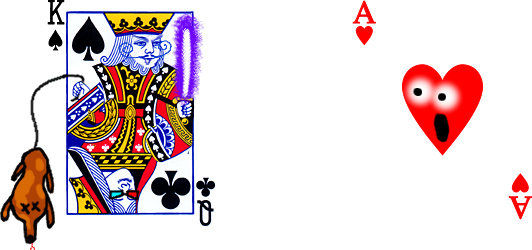
\includegraphics[width = \textwidth]{../logo.png}
	\end{center}

	\vfill

	% License
	% This file is part of Combo Whist.
%
% Copyright 2014-2019 Joakim Nilsson
%
% This file is part of Combo Whist.
%
% Combo Whist is free software: you can redistribute it and/or modify
% it under the terms of the GNU General Public License as published by
% the Free Software Foundation, either version 3 of the License, or
% (at your option) any later version.
%
% Combo Whist is distributed in the hope that it will be useful,
% but WITHOUT ANY WARRANTY; without even the implied warranty of
% MERCHANTABILITY or FITNESS FOR A PARTICULAR PURPOSE.  See the
% GNU General Public License for more details.
%
% You should have received a copy of the GNU General Public License
% along with this text.  If not, see <http://www.gnu.org/licenses/>.
% License notice

\begin{verbatim}
	Copyright 2007-2019 Joakim Nilsson

	This document is part of Combo Whist.

	Combo Whist is free software: you can redistribute it and/or modify
	it under the terms of the GNU General Public License as published by
	the Free Software Foundation, either version 3 of the License, or
	(at your option) any later version.

	Combo Whist is distributed in the hope that it will be useful,
	but WITHOUT ANY WARRANTY; without even the implied warranty of
	MERCHANTABILITY or FITNESS FOR A PARTICULAR PURPOSE.  See the
	GNU General Public License for more details.
\end{verbatim}
\verb|You should have received a copy of the GNU General Public License|\\
\verb|along with this text.  If not, see <|\url{http://www.gnu.org/licenses/}\verb|>.|


	\thispagestyle{empty}
	\pagebreak

	% Table of contents and list of tables without protrusion
	\microtypesetup{protrusion=false}
	\setcounter{tocdepth}{3}
	\tableofcontents
	\listoftables
	\microtypesetup{protrusion=true}
	\thispagestyle{empty}
	\pagebreak
}


% Change em dash to en dash in section references
\renewcommand{\sectionref}[1]{%
	\ref{sec:#1} -- \nameref{sec:#1}%
}

% Title
\defTitle{Kombinations-Whist}{Det Obesudlade Kortspelet}

% Links text
\defLinks{För den senaste versionen av reglerna, besök \rulesUrl\ eller prenumerera på \rssUrl.}

% Author
\author{Av Joakim Nilsson}

% Date and version
\ifdefined\varDev
	\date{Utvecklingsversion (baserad på version \varVersion-\varLanguage) -- \today}
\else
	\date{Version \varVersion-\varLanguage\ -- \today}
\fi

% Document
\begin{document}
	%=============
	% Intro pages
	%=============

	\introPages
	\pagebreak

	%======
	% Body
	%======

	\section{Översikt}
	Whist-varianten Kombinations-Whist är ett kortspel som bygger på sticktagande. Det är lätt att lära sig på några minuter, men svårt att bemästra.

	I Kombinations-Whist presenteras spelarna med en exceptionellt stor uppsjö av möjligheter till olika spelsätt genom att låta dem förhandla om en kombination av regler att använda inför varje hand. Detta genomförs genom att spelarna presenteras med ett \emph{någorlunda litet antal bud} som kan kombineras på ett \emph{stort antal sätt} till ett så kallat kombinations-bud, vilket bestämmer reglerna. Detta görs i hopp om att de stora möjligheterna till att styra reglerna på ett sofistikerat sätt gynnar skicklighet i motsats till slump mer än i andra Whist-varianter, utan att göra spelet onödigt komplicerat -- så att det ska vara roligt att spela både för nöjes- och professionella spelare.

	\paragraph{Antal spelare:}
	4 är att föredra, men 3 till $\infty$ går också bra med vissa regeljusteringar.

	\paragraph{Vad som behövs för att spela:}
	En standard-kortlek med 52 kort, samt penna och papper.

	\paragraph{Kortens rang:}
	Från högst till lägst: E, K, D, Kn, 10, 9, 8, 7, 6, 5, 4, 3, 2

	\section{Hur man spelar}
	\subsection{Förberedelser}
	Om bara 3 spelare deltar, ta ut $\clubsuit 7$, samt alla 8:or, 9:or och 10:or från leken, så att 4 färger om 10, 10, 10, respektive 9 kort blir kvar.

	Gör en kolumn för varje spelare på pappret. Detta görs för att hålla koll på poängställningen och lite annan information om spelet. När pappret är förberett, slumpa fram vem som blir giv.

	\subsection{Given}
	En giv består av två huvudsakliga delar -- \emph{budgivningen} och \emph{handen}. Eftersom det borde bli lättare att förstå budgivningen om spelet redan beskrivits, beskrivs spelet först.

	En giv börjar med att given delar ut 13 kort till varje spelare. Därefter börjar budgivningen, och när den är avklarad börjar spelet.

	Efter spelet noteras spelarnas poäng och en ny giv börjar där spelaren till vänster om föregående giv blir ny giv.

	\subsubsection{Handen}
	Handen spelas likt i de flesta Whist-varianter: Spelaren till höger om \emph{spelföraren}\footnote{Begreppet ''spelförare'' förklaras i Stycke~\sectionref{bidding}.} kallas \emph{förhand} och börjar med att spela ut ett kort. Därefter spelar övriga spelare ett kort var i medsols turordning. De övriga spelarna måste -- om de kan -- spela kort som följer förhands färg. Kan de inte det måste de saka valfritt kort eller spela trumf. Till skillnad från vissa Whist-varianter finns inget trumftvång ifall en spelare har slut kort i den utspelade färgen.

	Den spelare som spelade det högsta kortet i den först utspelade färgen tar hem \emph{sticket}\footnote{Det vill säga tar alla utspelade kort och lägger på bordet dem med bildsidan nedåt.} såvida ingen har spelat ut en trumf. Om så skulle vara fallet är det den spelare som spelade ut den högsta trumfen som tar hem sticket. Den spelare som tog hem det senaste sticket spelar ut i nästa stick.

	\subsubsection{Budgivningen}
	\label{sec:bidding}
	I Kombimations-Whist budar man med \emph{kombinations-bud}. Ett kombinationsbud består av exakt ett standardbud och en valfri mängd unika specialbud, inklusive noll. Till de olika buden tillkommer särskilda regler, vilka tillämpas under handen och poängberäkningen.

	Spelarna budar medsols och spelaren till vänster om given budar först. En spelare kan antingen buda ett kombinationsbud med högre rang än föregående kombinationsbud, eller passa. En passande spelare passar åker ut ur budgivningen och får därför inte lägga några nya bud förrän nästa giv. Om alla spelare passar blir det omgiv där samme giv ger igen.

	Ett kombinationsbuds rang utgörs av summan av rangen för alla ingående standard- och specialbud. För att ett bud ska få budas måste det minst vara av rang 1.

	Det föreslås att en tidsgräns på 30 sekunder sätts mellan varje bud med ytterligare 60 sekunder före det första budet. För nybörjare rekommenderas dock längre eller inga tidsgränser. En spelare som inte har lägger nåt bud inom den givna tiden passar automatiskt. Budgivningen fortsätter fram till att alla spelare förutom en har passat. Den icke-passande spelaren utnämns till spelförare varefter handen börjar.

	De standard- och specialbud som finns att tillgå finns listade i tabellerna i Stycke~\sectionref{standardBids}, respektive Stycke~\sectionref{specialBids}. Antalet stick att ta hem för att ett kombinationsbud ska gå hem listas i standardbudstabellens stickkolumn. Ett specialbud kan inte kombineras med ett annat bud som finns listat i dess inkompatibilitetskolumn. I övrigt är kombinationsbud som omöjligen kan gå hem oavsett budarens motspelares kortfördelning förbjudna.

	Om det är oklart när en händelse som inträffar på grund av ett bud ska ske, se specialbudens prioritetsskolumn. Ett buds prioritetsnummer bestämmer i vilken ordning de olika händelserna som ges av dess regler ska ske. De bud med lägst prioritetsnummer sker först. Alla standardbud har prioritetsnummer 0.

	\subsubsection{Poängberäkningen}
	Efter att handen har spelats klart uppdateras spelförarens poängsumma baserat på vilket kombinationsbud som lagts och huruvida detta bud gått hem. Om budet gick hem får spelföraren det antal poäng som specificeras i poängkolumnen för standardbudet. Om budet inte gick hem så förlorar spelföraren 2 poäng. En spelare kan anta en negativ poängsumma, men om en spelare innehar en poängsumma under $-5$, så tillåts denne inte att delta i budgivningar. Denne får dock 1 gratispoäng efter varje giv som denne deltar i (även i händelse av att ingen budar och det blir omgiv).

	\subsubsection{Vem som vinner}
	\label{sec:winning}
	Det finns två varianter för att bestämma vem som vinner i Kombinations-Whist: \emph{klassisk} och \emph{begränsad}.

	\paragraph{Klassisk:}
	Den som först uppnår eller överstiger \emph{vinstsumman} vinner. Vinstsumman börjar på 13, men minskar med 1 varje gång alla spelare har varit giv en gång vardera -- efter varje \emph{runda}. Detta fortgår fram till dess att vinstsumman går ned till 1, där den stannar fram till dess att någon vinner. Vinstsumman minskar \emph{efter} att poängen för den handen räknats. En spelare kan endast vinna genom att ett bud går hem och kan därför inte vinna enbart därför att vinstsumman minskar. En spelare kan inte heller vinna om denne inte innehar enskilt flest poäng.

	\paragraph{Begränsad:}
	Ett förutbestämt antal rundor spelas (förslagsvis 3). När alla rundorna har spelats vinner näste spelare som går hem med ett bud som resulterar i att denne uppnår enskilt flest poäng. För att förtydliga: En spelare kan vinna i samband med att sista rundan just spelats färdigt.

	\paragraph{Skamvinst} Gemensamt för bägge varianterna gäller att om alla spelare utom en innehar $-5$ poäng eller färre så vinner den spelare som har flest poäng. Detta sätt att vinna kallas en \emph{Skamvinst}.

	\section{Övrigt}
	\subsection{Regler för fler än 4 spelare}
	Om fler är 4 spelare deltar i spelet så får alla utom 4 sitta ut (avstå att delta) i en giv. De spelare sitter närmast till höger om given sitter ut.
		
	\subsection{Prat}
	Spelarna får prata på så länge de inte ger några ledtrådar om vilka kort de besitter.
		
	\subsection{Fusk}
	Om spelföraren oavsiktligen fuskar går nuvarande bud inte hem. Om en icke-spelförare oavsiktligen fuskar händer följande: Det nuvarande budet spelas klart, men inget poängavdrag görs från spelförarens poängsumma utifall budet inte går hem. Dessutom dras samma antal poäng som det nuvarande budets poäng av från den fuskande spelarens poängsumma oavsett om budet går hem.

	Om oavsiktligt fusk inträffar innan en spelförare har utnämnts avbryts given och 2 poäng dras av från den fuskande spelarens poängsumma.

	Om givens samtliga spelare emellertid är överens om hur händelserna efter fusket inträffade ska kompenseras ska detta dock ske utan andra förändringar i poängsummorna förutom att 1 poäng dras av från den fuskande spelarens poängsumma.

	En spelare som avsiktligen fuskar i Kombinations-Whist får aldrig mer spela det eftersom denne uppenbarligen inte respekterar spelets prakt.

	%============
	% Bid tables
	%============

	\pagebreak
	\newgeometry{left=1cm, right=1cm, top=1cm}

	\section{Standardbud}
	\label{sec:standardBids}
	\begin{center}
		\begin{tabularx}{\textwidth}{
				p{2.5cm}
				S[table-number-alignment=center, table-format=1.0]
				S[table-number-alignment=center, table-format=1.0]
				ccX
			}
			\textbf{B\scriptsize ENÄMNING} &
			\rotccw{\textbf{Rang}} &
			\rotccw{\textbf{Poäng}} &
			\rotccw{\textbf{Trumf}} &
			\rotccw{\textbf{Stick}} &
			\textbf{Regler}
			\\[-3ex]

			\directlua{tableItemsStandardBids()}
		\end{tabularx}
	\end{center}

	\newcommand{\nonTrump}{\textnormal{trumflösa bud}}
	\section{Specialbud}
	\label{sec:specialBids}
	\begin{center}
		\begin{tabularx}{\textwidth}{
				p{2.1cm}
				S
				S
				p{2.7cm}
				X
			}

			\textbf{B\scriptsize ENÄMNING} &
			\rotccw{\textbf{Rang}} &
			\rotccw{\textbf{Prioritet}} &
			\textbf{Inkompatibilitet} &
			\textbf{Regler}
			\\[-3ex]

			\directlua{tableItemsSpecialBids()}
		\end{tabularx}
	\end{center}
\end{document}
